\chapter{Background Knowledge}
To formulate a multi-robot search problem, some preliminaries are introduced.
Submodularity (Def. \ref{def:defsubmodular}) and independence system (Def. \ref{def:independence-system}) are adopted to formulate the objective function and the robot constraints, respectively.
The objective function consists of the coverage and balancing function (Thm. \ref{thm:proposed-obj}).
The constraint includes clustering of the search environment (Thm. \ref{thm:clustering-matroid}).
The advantage of formulating the submodular maximization subject to the intersection of an independence system (Thm. \ref{thm:intersection-k-systems}) is that the theoretical guarantee is given (Thm. \ref{thm:intersection-matroid-bound}).
To further improve the performance, Def. \ref{def:matroid} introduces the concept of matroid.\\


\section{Submodularity}

The definition and illustration of submodularity are as follows:

\begin{definition} \label{def:defsubmodular} (Submodularity) \cite{nemhauser1978analysis}
A function $f:2^N \rightarrow \mathbb{R}^+$ is submodular if and only if $\forall S \subseteq T \subseteq N, \forall e \in N \setminus T, \ f(S\cup \{e\}) - f(S) \geq f(T\cup \{e\}) - f(T)$. \\
\end{definition}

Let $S=\{1,2,3\}$ be the ground set and $S_A=\{1\}$, $S_B=\{1,2\}$ be two different sets selected from the ground set, i.e., $S_A \subseteq S_B \subseteq S$. In Fig. \ref{submodularity} (a)(b), if the submodular function $f$ is defined as the coverage function, $f(S_A)$ and $f(S_B)$ depict the regions observed by the camera FOV at locations of $\{1\}$ and $\{1,2\}$.
When a new set $s=\{2\}$ is added to both $S_A$ and $S_B$, the marginal gain of the coverage function $f$ is the additional regions covered, which is the red dashed line area shown in Fig. \ref{submodularity}(c). The diminishing return property suggests that incorporating a set into the smaller set results in a greater marginal gain.\\

%\begin{figure}[htbp]
% \begin{center}
%\begin{subfigure}{.22\textwidth}
%  \centering
%  
\includegraphics[width=1.0\linewidth]{sub6.eps}
%  \caption{$F(S_A)$}
%\end{subfigure}
%\begin{subfigure}{.22\textwidth}
%  \centering
%  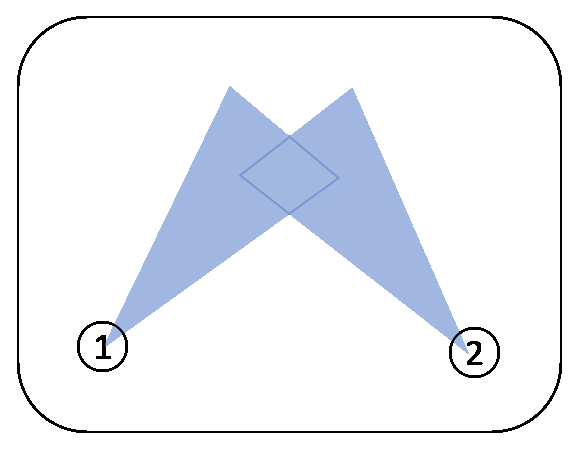
\includegraphics[width=1.0\linewidth]{sub7.eps}
%  \caption{$F(S_B)$}
%\end{subfigure}
%\begin{subfigure}{.44\textwidth}
%  \centering
%  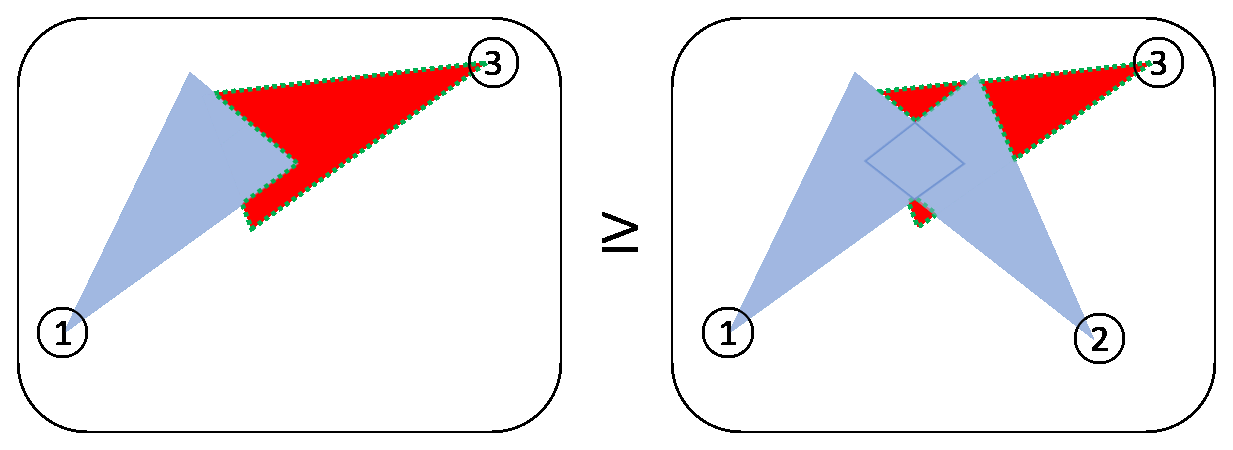
\includegraphics[width=1.0\linewidth]{sub5.eps}
%  \caption{$F(S_A \cup s)-F(S_A)$ and $F(S_B \cup s)-F(S_B)$}
%\end{subfigure}
%\caption{Illustration of submodularity. The decimal number represents the selected sensor.
%The colorful and white areas represent the covered and uncovered areas, respectively.
%(a) $F(S_A)$ represents the covered area by $S_A,$ where $S_A = \{1\}.$ (b) $F(S_B)$ represents the covered area by $S_B,$ where $S_B = \{1, 2\}.$
%(c) The green dash lines represent the submodular gain after adding $s,$ where $s = \{3\}.$ Left figure shows the $F(S_A\cup s) - F(S_A)$ and right figure shows that $F(S_B\cup s) - F(S_B).$}
%\label{fig:submodularity}
% \end{center}
% \end{figure}

\section{Matroid}

\begin{figure}
   \centering
   \begin{subfigure}[b]{0.3\textwidth}
       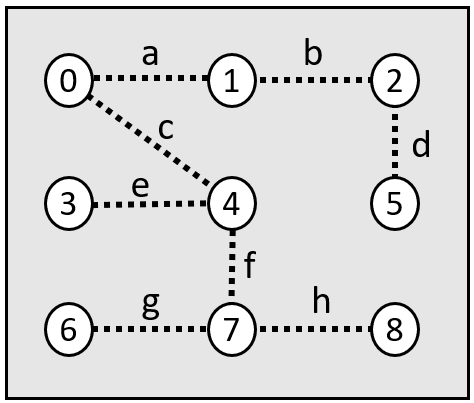
\includegraphics[width=1\textwidth]{def-mat-0.png}
       \caption{Ground set $E$}
   \end{subfigure}
   \hfill
   \quad
   \centering
   \begin{subfigure}[b]{0.3\textwidth}
       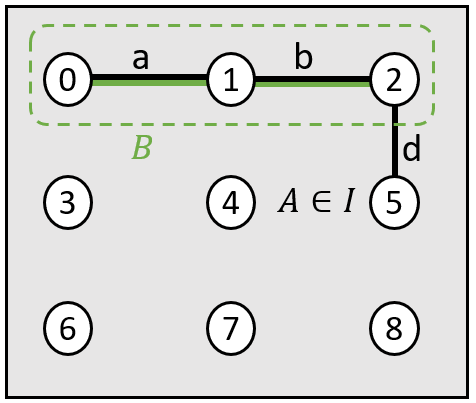
\includegraphics[width=1\textwidth]{def-mat-1.png}
       \caption{$A \in \mathcal{I}$ and $B \subseteq A$}
   \end{subfigure}
   \hfill
   \quad
   \begin{subfigure}[b]{0.3\textwidth}
   \centering
       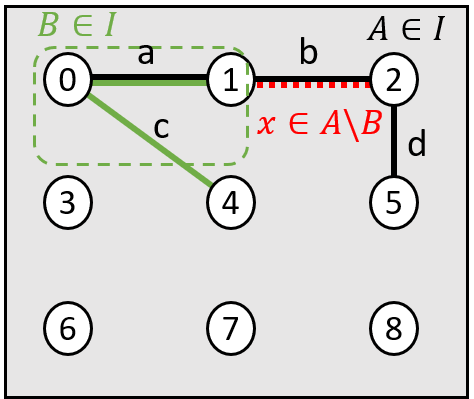
\includegraphics[width=1\textwidth]{def-mat-2.png}
       \caption{$|A|>|B|$}
   \end{subfigure}
   \hfill

   \caption{Illustration of the downward closure and the exchange property.
   The vertices represent the geographic locations of sensors, and the edges are the distance between two vertices. (a) The ground set $E=\{a,b,c,d,e,f,g,h\}$ (the black dashed lines) (b) $A=\{a,b,d\}$ (the black solid lines) is a set that satisfies the independent set $\mathcal{I}$. $B=\{a,b\}$ (the green solid lines) is a subset of $A$.
   (c) Two sets $A=\{a,b,d\}$ (the black solid lines) and $B=\{a,c\}$ (the green solid lines) satisfy the independent set $\mathcal{I}$, where $|A|>|B|$. Then there exists an element $x \in A \setminus B$ such that adding to the smaller set $B$ still satisfies the condition of the independent set $\mathcal{I}$, e.g., $x=b$ (the red dashed lines).
   }
   \label{def-matroid}
\end{figure}

\begin{definition} \label{def:independence-system} (Independence System) \cite{korte1978analysis}
An independence system is a pair $(E, \mathcal{I})$, where $E$ is a finite set called the ground set and $\mathcal{I}$ is a family of subsets of $E$ called independent sets such that:
\begin{enumerate}
    \item (non-emptiness) $\emptyset \in \mathcal{I}$;
    \item (downward closure) if $A\in \mathcal{I}$ and $B \subseteq A$, then $B \in \mathcal{I}$. \\
\end{enumerate}

An illustrative example is as follows.
Consider a ground set $E=\{a,b,c,d,e,f,g,h\}$ and an independent set $\mathcal{I}=\{\{a,b,c\}, \{a,b,d\}, \{a,b\}, \\ \{a,c\}, \{a,d\}, \{b,c\}, \{b,d\}, \{a\}, \{b\}, \{c\}, \{d\}, \emptyset \}$, shown in Fig. \ref{def-matroid}(a).
Let $A \in \mathcal{I}$ be a set, and $B \subseteq A$ be a subset. In Fig. \ref{def-matroid}(b), the downward closure property states that if $A\in \mathcal{I}$ and $B \subseteq A$, then $B \in \mathcal{I}$.\\
\end{definition}

\begin{definition} \label{def:k-independence-system} ($k$-independence System) \cite{korte1978analysis}
Given a ground set $E$, an independence family $\mathcal{I}$ and a set $Y\subset E$. Let $r(Y)=\{A \in \mathcal{I} | A\subseteq Y \text{ and there is no }A' \in \mathcal{I} \text{ such that } A\subset A' \subseteq Y \}$. Then $(E, \mathcal{I})$ is a $k$-independence system if for all $Y\subset E$,
\begin{align*}
    \frac{\max_{A\in r(Y)}|A|}{\min_{A\in r(Y)}|A|} \leq k,
\end{align*}
where $k\geq1$ and $|\cdot|$ is defined as the number of elements. As a special case, if $k=1$, then $(E, \mathcal{I})$ is a matroid. \\
\end{definition}

To clarify the concept of $k$-independence system, consider a ground set $E=\{1,2,3,4,5\}$ and an independence family $\mathcal{I}=\{\{1,2,3\},\{1,2\},\\ \{1,3\},\{1,4\},\{2,4\},\{1\},\{2\},\{3\}, \{4\},\emptyset \}$. Let $Y=\{2,3,4\}$ be a subset of $E$. By definition, $r(Y)=\{\{3\},\{2,3\},\{2,4\},\{3,4\}$\}. The ratio of the maximal cardinality to the minimal cardinality is 2. Thus, $k\geq2$.

\begin{definition} \label{def:matroid} (Matroid) \cite{nemhauser1978analysis}
A matroid $\mathcal{M}$ is a pair $(E, \mathcal{I})$, where $E$ is a finite set called the ground set and $\mathcal{I}$ is a family of subsets of $E$ called independent sets, with the following properties:
\begin{enumerate}
    % \item (non-emptiness) $\emptyset \in \mathcal{I}$;
    \item (downward closure) if $A\in \mathcal{I}$ and $B \subseteq A$, then $B \in \mathcal{I}$;
    \item (exchange property) if $A \in \mathcal{I}, B\in \mathcal{I}$ and $|A|>|B|$, then there exists $x \in A\setminus B$ such that $B \cup \{x\} \in \mathcal{I}$.\\
\end{enumerate}
\end{definition}

An example of a matroid $\mathcal{M}=(E, \mathcal{I})$ is illustrated in Fig. \ref{def-matroid}.
Consider a ground set $E=\{a,b,c,d,e,f,g,h\}$ and an independent set $\mathcal{I}=\{\{a,b,c\}, \{a,b,d\}, \{a,b\}, \{a,c\}, \{a,d\}, \{b,c\}, \{b,d\}, \{a\}, \\ \{b\}, \{c\}, \{d\}, \emptyset \}$ in Fig. \ref{def-matroid}(a).
Let $A \in \mathcal{I}$ be a set and $B \subseteq A$ be a subset, shown in Fig. \ref{def-matroid}(b). The downward closure property states that if $A\in \mathcal{I}$ and $B \subseteq A$, then $B \in \mathcal{I}$. In Fig. \ref{def-matroid}(c), consider two sets $A \in \mathcal{I}$ and $B \in \mathcal{I}$, where $|A|>|B|$. By the exchange property, there exists an element $x \in A\setminus B$ such that $B+x \in \mathcal{I}$.\\

\begin{theorem} \label{thm:intersection-k-systems} (Intersection of independence systems) \cite{mestre2015intersection}
The intersection of a $k_1$-independence system and a $k_2$-independence system is a $(k_1 + k_2)$-independence system. \\
\end{theorem}

To illustrate the concept, let $(E, \mathcal{I}_1)$ and $(E, \mathcal{I}_2)$ be a $k_1$-independence system and a $k_2$-independence system, respectively.
The goal is to find the intersection of $(E, \mathcal{I}_1)$ and $(E, \mathcal{I}_2)$, namely $(E, \mathcal{I}_1 \cap \mathcal{I}_2)$. Then $(E, \mathcal{I}_1 \cap \mathcal{I}_2)$ is a $(k_1 + k_2)$-independence system. \\

\begin{theorem} \label{thm:intersection-matroid} (Intersection of matroids) \cite{nemhauser1978analysis}
Consider the matroid intersection system

\begin{align} \label{eq:inter-matroid}
    \bigcap_{\mathcal{M}\in \mathit{\mathbb{M}}} \mathcal{M} \triangleq\left ( \mathcal{V},\ \bigcap_{\mathcal{M}\in \mathit{\mathbb{M}}} \mathcal{M} \right )
\end{align}

where $\mathit{\mathbb{M}}$ is a set of matroidal independence systems, $\mathcal{M}$ is a matroid, and $\mathcal{V}$ is a ground set. Eq. \eqref{eq:inter-matroid} models any arbitrary independence system. \\
\end{theorem}

\begin{theorem} \label{thm:intersection-matroid-bound} (Theoretical bound of a matroid intersection) \cite{fisher1978analysis}
Given a submodular monotone set function $F$ and a set of matroidal independence systems $\mathit{\mathbb{M}}$, maximizing $F$ under an intersection of matroids with the greedy algorithm yields a solution $X$. The performance of the set $X$ is

\begin{align*} \label{eq:inter-matroid}
    F(X) \geq \frac{1}{|\mathit{\mathbb{M}}|+1} F(X^{opt}),
\end{align*}
where $|\mathit{\mathbb{M}}|$ is the cardinality of $\mathcal{M}$ and $X^{opt}$ is an optimal solution. \\
\end{theorem}

Consider a set of matroidal independence systems $\mathit{\mathbb{M}} = \{\mathcal{M}_1, \mathcal{M}_2\}$.
The cardinality of $\mathit{\mathbb{M}}$ is $2$.
Therefore, greedy algorithms find a solution $X$ such that the performance of $X$ achieves $\frac{1}{3} F(X^{opt})$.\\

In multi-robot search scenarios, the search environment must be partitioned into smaller segments to accommodate multiple robots.
Ensuring an equitable distribution of workloads among robots is a key consideration for efficient task assignments.
Therefore, the coverage and balancing function \cite{li2024mrsis} and the clustering constraint \cite{liu2013entropy} are introduced. \\

\begin{theorem} \label{thm:clustering-matroid} (Clustering constraint) \cite{liu2013entropy}
Let $E$ be the edge set and $S \in E$ be the set of subsets. $\mathcal{M}_C=(E, \mathcal{I}_C)$ is matroidal, where $\mathcal{I}_C=\{S \subseteq E : N \geq n \}$, $N$ is the number of clusters, and $n$ is the clustering budget. \\
\end{theorem}

\begin{theorem} \label{thm:proposed-obj} (Submodularity of a coverage and balancing function) \cite{li2024mrsis}
Let $S$ be a set, $\lambda \in [0,1]$ be a constant, $f:2^S \rightarrow \mathbb{R}^+$ be a coverage function, and $\mathcal{B}: 2^S \rightarrow \mathbb{R}^+$ be a balancing function.
The coverage and balancing function $F(S)=f(S)+\lambda \mathcal{B}(S)$ is submodular. \\
\end{theorem}

\begin{theorem} \label{thm:balance} (Submodularity of balancing function) \cite{liu2013entropy}
 Given a graph $\mathcal{G}=(V, E)$ and a partition set $S=\{S_i \in V : i\in \{1,...,N\}\}$, the balancing function $\mathcal{B}:2^E \rightarrow \mathbb{R}$ is a monotonically increasing submodular function and is defined as follows:
 \begin{align*}
     \mathcal{B}(S)=-\sum_{i} {p_S(i)\log({p_S(i)})-N},
 \end{align*}
 where $p_S(i)=\frac{|S_i|}{|V|}, i=\{1,...,N\}$ and $N$ is the number of connected components in the graph.

 The balancing function encourages the clusters to have similar sizes. Fig. \ref{balancing-func} shows the balancing function of two topologies. The balancing function shown in Fig. \ref{balancing-func}(a) has a higher value compared to that in Fig. \ref{balancing-func}(b). In other words, the higher balancing value has more balanced clustering.\\
\end{theorem}

\begin{figure}
    \centering
    \begin{subfigure}[b]{0.4\textwidth}
    \centering
        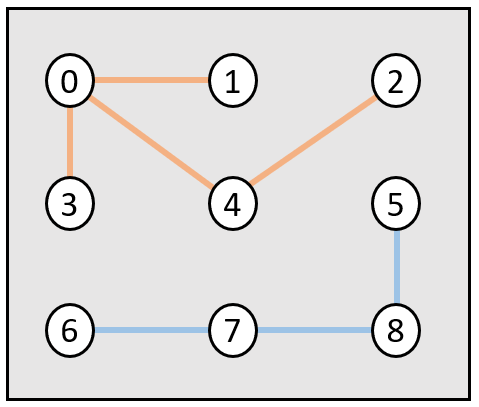
\includegraphics[width=1\textwidth]{-1.01.png}
        \caption{$\mathcal{B}(S_A)=-1.01$}
    \end{subfigure}
    \hfill
    \quad
    \begin{subfigure}[b]{0.4\textwidth}
        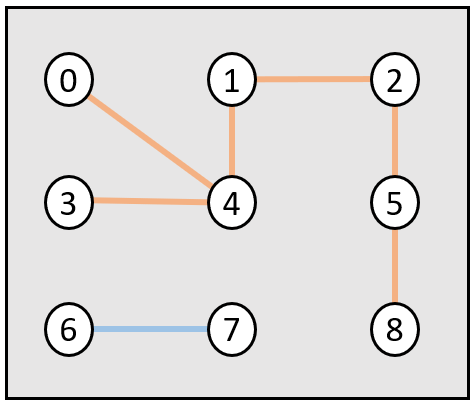
\includegraphics[width=1\textwidth]{-1.24.png}
        \caption{$\mathcal{B}(S_B)=-1.24$}
    \end{subfigure}
    \hfill

    \caption{Illustration of the balancing function. Two clusters are denoted by orange and blue colors. (a) $\mathcal{B}(S_A)$ is the balancing value of $S_A$, where $S_A=\{S_1,S_2\}$, $S_1=\{0,1,2,3,4\}$ and $S_2=\{5,6,7,8\}$. (b) $\mathcal{B}(S_B)$ is the balancing value of $S_B$, where $S_B=\{S_1,S_2\}$, $S_1=\{0,1,2,3,4,5,8\}$, and $S_2=\{6,7\}$.
    }
    \label{balancing-func}
\end{figure}

